\chapter{Hypertext + Markup + Information + Semantics = HTML}
\label{html}
\paragraph{} In this chapter we will study our first web language, the HyperText Markup Language (HTML). During our study we will consider the various historical versions of HTML and their impact upon the modern web, then focus on HTML 5 and the production of modern semantic HTML as the core of our websites.
\paragraph{} HTML is one of the three core technologies of the Web,the other technologies being Cascading Style Sheets (CSS) and JavaScript (JS). We will cover all of these technologies during this module, but need to start somewhere. All three technologies are languages but they each target a different aspect of the Web, they each work together in different ways, and they each have different powers in terms of what they can be used to do and what their limits are.
\paragraph{} Of the three technologies, the best place to start is with HTML. This is because every site has some underling HTML, even if this is subsequently discarded and entirely replaced with a site generated on-the-fly using JavaScript. There is always a minimal page that hosts the other languages and gives the browser a starting place for deciding what to display. For example, open a new, empty, browser window and then use the browser developer tools to inspect the page that is displayed. The browser gives you a default empty page. This empty page is described using HTML. We can conclude therefore that HTML is both critical and central to the functionality of the Web.
\paragraph{} In the last unit we talked about the idea of HyperText and how this facilitates links between pages. In addition to this we also need to consider that links without content don't give us much, our pages need to have some content to display that the links can depict relationships between. One way to describe page content is through markup, the use of tags to "mark-up" or delineate sections of the page, such as a word or phrase or other string of text, that should be treated differently from the rest of the page. What is it that is marked-up? It is content, or information. Finally what is it we are trying to convey through web pages. We are not merely distributing information, there are other formats we could use if it was just about sharing information, e.g. database formats and file formats, but web pages try to convey content that has meaning, content that has meaning in the context of the other content that surrounds it. When we talk about meaning we often use the term semantics. 
\paragraph{} So if we put these four aspects together, we get the title of this unit:\\
{\bf{Hypertext + Markup + Information + semantics = HTML}}

\section{HTML \& The Web}
\paragraph{} HTML is generally stored on Web servers and processed by Web browsers. You should consider this in the context of our overview of the Web and networking concepts in the last unit. This is not the only way to use HTML, but it is probably the most common at the moment.
\paragraph{} The Web was designed for ease of publication - a non-programmer, such as a physicist or other research scientist should be able to develop and deploy Web-sites and Web-pages without needing to write (much) code. Technically, writing a Web page using HTML is a form of coding, you are using a language to tell a piece of software what to do. However, this language is so restricted and focused so carefully on its target, representation of documents, that it is usable by a wide section of society. Think about it, most literate people are able to identify a heading from other pieces of text, or to pick out a paragraph or other document-oriented organisational unit. This is all that people really do when they are making an HTML document.
\paragraph{} It helps also that browsers are quite good at taking malformed HTML documents and repairing them, or at least doing the best they can to display the content. This can mean that the content doesn't quite appear the way the writer intended, but at least it can, usually, be displayed. To achieve this browsers have traditionally been very accommodating in what they will accept, not only in terms of malformed HTML, but also in terms of older versions of HTML.
\paragraph{} Many sites are also very long lived. We don’t want to break sites just because a newer version of HTML, CSS, JS, \&c. is available. So browsers are usually very backwards compatible. They are  generally capable of rendering very old sites. Note however that some technologies have lived and died along the way and some browsers, usually for security and stability reasons, have stopped supporting some technologies. Flash is a good example of such a "dead" technology. However the core languages, HTML, CSS, and JS are still, and probably always will be, supported.
\paragraph{} As a result, you will see code from lots of versions of the Web and should be in a position to handle it (HTML in general) but we should aim to develop using the latest tools (e.g. HTML5) - particularly because HTML 5 (semantic HTML) added organisational elements that are distinct from previous versions. This is why we are covering bother HTML in general in this unit, but also HTML5. We want to be able to cope, as professionals, with older versions, but also to create modern new sites.

\section{HTML}
\paragraph{} Having considered the relationship between HTML and the Web we can now perhaps concentrate on HTML itself. We've already said that HTML is the HyperText Markup Language. That is, a  language for turning text into hypertext by using markup. Note though, that in the grand scheme of things, this is just one way of creating hypertext and not the only way to create hypertext. It is perhaps the most dominant although you might have also experienced alternatives like markdown. In older word processors you used to be able to turn on the display of markup because word processor documents are similarly marked up, albeit internally, to indicate the different parts of the document. In some ways a word processor is very similar, in some contexts, to a Web browser. The underlying format for Microsoft Word documents is an XML document. XML is the eXtensible Markup Language so you'll find markup in lots of places once you know what to look for.
\paragraph{} HTML is the standard markup language for creating web pages. It is not a programming language  though. This is because it doesn't have any support for programming constructs like expressions, looping, or iteration, i.e. you can't write general purpose programs in HTML. What you can do though is define a Web page.
\paragraph{} HTML is just one part of the triad of foundational web technologies (alongside CSS and Javascript). We use it to describe the semantic structure of the data, which CSS in turn presents, usually visually, to the user, and which Javascript can manipulate. 
\paragraph{} Generally HTML arrives in the browser via one of two routes, either from local storage or from a server. From a server is the most usual. Opening a document from local storage is what happens when you open an HTML file on your local computer, for example, by double clicking an HTML file. A file opened from local storage will run with reduced capability than one requested from a Web server. This is due to security policies associated with web browsers. You don't want your browser to have unrestricted access to your local file system when running arbitrary code, such as HTML which might have embedded or linked JS. The other route, requesting a page from a web server is more usual and is likely the most dominant method for getting a page to display in a browser. This happens after a successful request-response cycle between the browser and the web server. 
\paragraph{} Once the browser receives an HTML document from either server or storage it then renders that document visually. Note that other user agents can retrieve HTML may use the returned HTML in other ways, for example, rendering the content as spoken text or via a braille display for visually impaired users.

\section{What dos AN HTML Document look like?}
\paragraph{} We've talked a bit about these HTML documents and how to retrieve them, but what do they actually look like?
\paragraph{} Well, something like this (depending upon the content that is marked up, which is basically unlimited):
\begin{lstlisting}
	<!DOCTYPE html>
	<html>
		<head>
			<title>My first HTML 5 document</title>
		</head>
		<body>
			<p>Hello World from HTML 5</p>
		</body>
	</html>
\end{lstlisting}

\paragraph{} Remember that HTML is plain text. This means that you can write HTML in any text editor and only need to save it as a .html document (which can then be opened in a browser).  Most operating systems will take care of the details of opening the file correctly. Depending upon your setup though you might need to specifically tell your machine to open an HTML document either in your browser or your editor, depending upon which you do most often. I find myself that HTML files on my local storage are usually there for editing so I have my machine set up to open files ending in .html (and .css and .js for that matter) in my favourite text editor rather than in my default web browser. Note that this doesn't affect your browsers ability to open and render HTML from web servers, or any file that is explicitly opened in the browser, i.e. via the File $>$ Open File menu item or a dragged and dropped file.

\section{Classical HTML to Modern HTML}
\paragraph{} We are currently on version 5 of HTML, known as HTML5, but there have been multiple major and sub-versions of HTML over the last thirty years or so. A lot of web sites are still written, and are still being written, using earlier versions of HTML. So it is worth your while to be aware of earlier versions and how and why they changed. Also, remember that HTML has developed over the years, usually in response to the desires of users and designers who are generally trying to make the Web better.
\paragraph{} Early versions of HTML, at least until version 4.01 were primarily concerned with defining the visual presentation of a web page. This mixed both structure and presentation. That is the structure of a page, such as whether a section of text is a heading or a paragraph, but also how that section of text should look to the user, e.g. the font face, font size, font colour, etc.
\paragraph{} If we think about how an HTML page can be used in different ways, either viewed in a browser, or processed for use in other tools, or in a mobile app, or an accessibility device like a Braille reader, or rendered differently for printing to paper or saving to a PDF, then it seems silly to dictate in the HTML how the page should look, because that depends on how it is being used, and that decision, no matter how much a designer might want to control things, is a decision for the end user to make. As a result, over time the HTML language has been revised to remove the aspects that deal with presentation and concentrate solely on structure and meaning. Presentational aspects have, instead, become the responsibility of a language designed for it, namely CSS.
\paragraph{} So modern HTML describes the content, its structure, and its relation to other content and visual presentation of those things is delegated to CSS.


\section{HTML ELEMENTS}
\paragraph{} HTML documents are constructed from HTML Elements. Let's consider our example HTML document from earlier:
\begin{lstlisting}
	<!DOCTYPE html>
	<html>
		<head>
			<title>My first HTML 5 document</title>
		</head>
		<body>
			<p>Hello World from HTML 5</p>
		</body>
	</html> 
\end{lstlisting}
\paragraph{}
The whole thing is an HTML document, but it is made from individual HTML elements. Elements are keywords that are encapsulated within angle brackets, e.g. $<$html$>$.

\paragraph{} Notice also that many of the elements come in pairs, in fact all of the elements in our example above. Elements are represented using opening and closing tags, e.g. $<$html$>$$<$/html$>$  such that $<$html$>$ is an opening tag and $<$/html$>$ is a closing tag. Most tags delineate the start and end of a portion of text or enclose other sets of tags so are often paired, one for each end of the section. 

\paragraph{} Some stand alone amongst the text, e.g. $<$br /$>$ which is used to insert a line break within a document. Standalone tags aren't part of an opening and closing pair, so aren't capable of enclosing a section of text or any other element like pairs do.

\paragraph{} Tags are combined to create structured documents by denoting structural semantics for the text (such as headings, paragraphs, lists, links, etc.). Notice how, in our example, everything is enclosed within the $<$html$>$ pair. The next layer of tags is the $<$head$>$ and $<$body$>$ pairs. The $<$head$>$ pair encapsulates the $<$title$>$ pair, and the $<$body$>$ pair encapsulates the $<$p$>$ pair. This encapsulation results in a hierarchical structure, formally a tree structure. We can describe an  HTML document as having a tree structure where the $<$html$>$ tags are the root of the tree, and the, in our example, $<$p$>$ and $<$title$>$ tags are the leaves of the structure.

\section{HTML Element Structure}
\paragraph{} HTML Elements are not just simple words with angle brackets around them like we saw in our example, e.g.
\begin{lstlisting}
	<p>Hello World from HTML 5</p>
\end{lstlisting}
\paragraph{}Elements can do so much more than that, for example, they can have attributes and values which can give the browser additional information about how to deal with the tag. For example, we can assign individual tags a class so that they can be grouped together. This is useful when we use CSS later as we can then say something like treat all tags in class x in this way, e.g. embolden all tags which are assigned to the important class, e.g. class="important". We can also give individual tags an ID so that they are uniquely identifiable and distinguishable from all other tags in the page. This is again useful when applying CSS and allows us to say, render this specific element, identified by ID, uniquely from everything else. Attributes and values are also used to attach javascript to individual elements so they are really important and give us one way to link between the various core web technologies and enable them to interact. 

\begin{figure}[H]
\centering
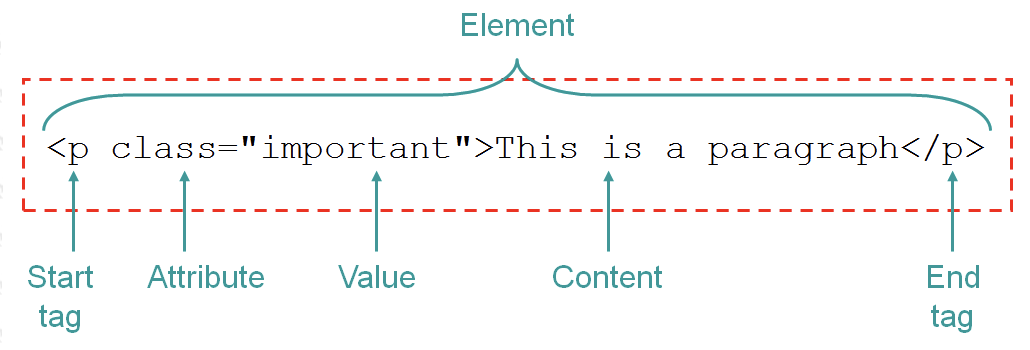
\includegraphics[width=0.8\textwidth]{figures/html-structure}
\label{fig:html-structure}
\end{figure}

\paragraph{} We'll see later that there are other methods we can exploit, but this is the core way at least from the perspective of HTML.

\section{HTML Versions}
\paragraph{} We mentioned earlier that there are various versions of HTML that you will come across. As you investigate various web pages you will notice considerable variation amongst versions of HTML . Having now considered the things that make up an HTML web page such as the tags, elements, and attributes, we can now inspect a simple comparison between HTML4.01 and HTML5.
\paragraph{} HTML4.01 looks like this:
\begin{lstlisting}
<!DOCTYPE HTML PUBLIC "-//W3C//DTD HTML 4.01//EN” 
	"http://www.w3.org/TR/html4/strict.dtd">
<HTML>
 	<HEAD>
      		<TITLE>My first HTML 4.01 document</TITLE>
  	</HEAD>
   	<BODY>
      		<P>Hello World from HTML 4.01</P>
   	</BODY>
</HTML>
\end{lstlisting}
\paragraph{} A very similar document using HTML5:
\begin{lstlisting}
<!DOCTYPE html>
<html>
	<head>
		<title>My first HTML 5 document</title>
	</head>
	<body>
		<p>Hello World from HTML 5</p>
	</body>
</html>
\end{lstlisting}
\paragraph{} A few things to note, HTML5 uses lowercase for tags which makes things generally easier to read. The DOCTYPE declaration is also much simpler and easier to remember than in HTML4.01. Otherwise things are fairly similar. The larger differences are in terms of the exact range of available tags available for each version. HTML5 deprecates certain tags that relate to styling, strengthens the semantic interpretation of other tags, and introduces a set of useful organisation tags that are purely concerned with the semantic relationship between tags and how those tags are grouped together. Over the new few sections we'll look at the rich range of HTML4.01 tags and then concentrate, towards the end of the unit, on the semantic aspects of HTML5.
\paragraph{} In summary, we should write HTML to the current version, e.g. HTML 5, but we should be aware of what earlier versions looked like so that we can handle them when we encounter them in the wild.

\section{Validity}
\paragraph{} Because HTML is a language we can talk about whether something written in that language is correct or not. If it is correct then it is valid and if it is incorrect then it is invalid. Think of this a bit like writing a sentence in English, or any other language, but we'll stick with English for now. We can write things in English that are not grammatically correct and this can lead people to not understand what we are trying to communicate to them. It is even more complex with most programming languages because people can be quite flexible in understanding each other but computers must be very precise in their use of language. Browsers are quite robust in their treatment of malformed HTML, but despite this, it is still better if our HTML documents are valid.
\paragraph{} There are tools to automatically verify that a given HTML document is correct (or otherwise) One example is the W3C validator tool\footnote{\url{https://validator.w3.org/}}:

\begin{figure}[H]
\centering
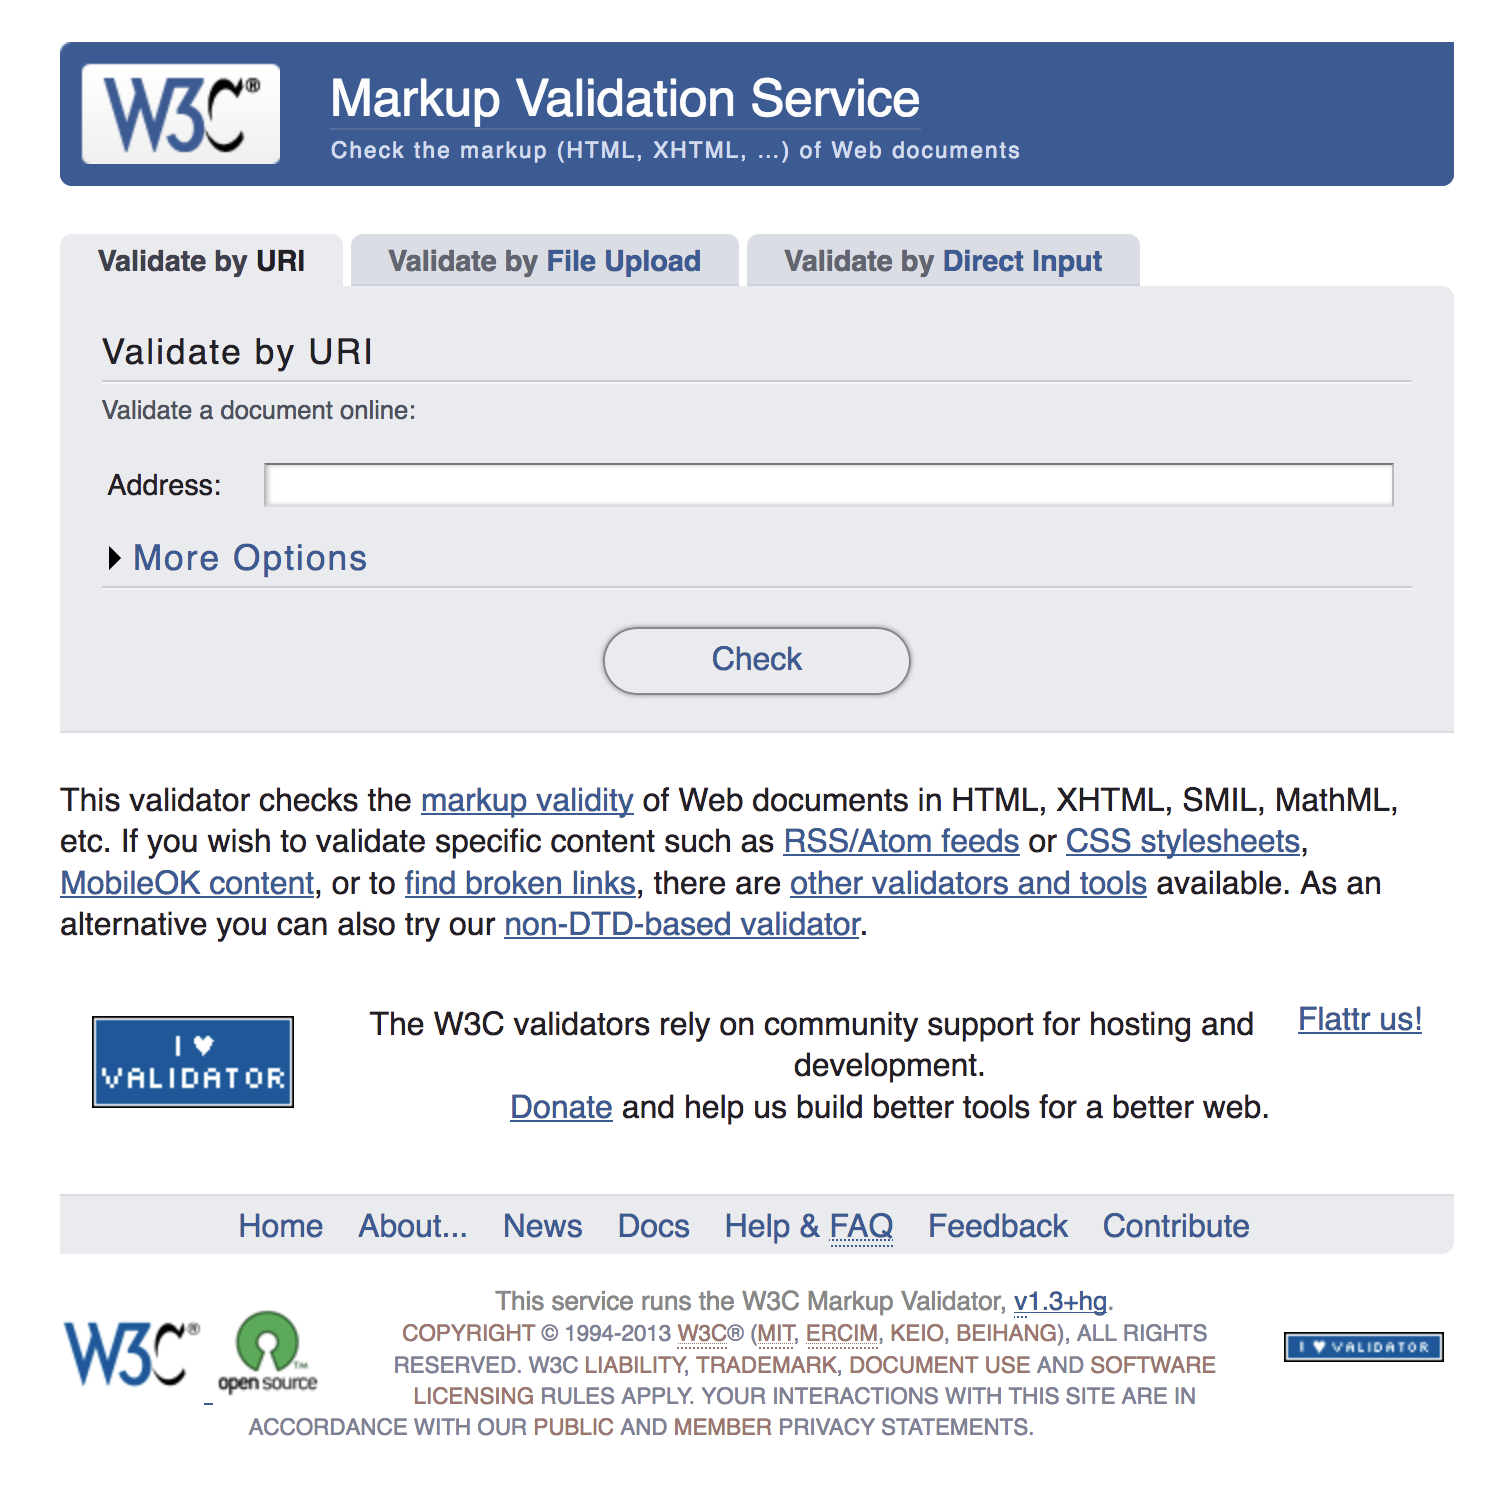
\includegraphics[width=0.8\textwidth]{figures/validation}
\label{fig:html-structure}
\end{figure}


\paragraph{} It is well worth testing pages that you write using this service, especially when you are first starting out with HTML.

\section{HTML Tags}
\paragraph{} We've mentioned HTML tags but haven't really examined the sheer range of tags that HTML has available. There are a large number of tags in HTML. This unit will survey many of them, but it is worth using the following resources to explore them in detail:
\begin{itemize}
\item MDN HTML Reference\footnote{\url{https://developer.mozilla.org/en-US/docs/Web/HTML/Element}}
\item W3Schools HTML Examples\footnote{\url{https://www.w3schools.com/tags/}}
\end{itemize}

\paragraph{} Let's try to take a structured approach to exploring the range of tags. Starting at the highest level we have an HTML document that contains a definition tag and structural tags. The structural tags can then contain other tags, frequently in combination and encapsulated within each other. Let's now survey the range of standard HTML tags.
\begin{description}
\item [Document Type Definition:] $<$doctype$>$
\item [Document Structure:] $<$html$>$$<$head$>$$<$body$>$
\item [Within the $<$head$>$ section:] $<$title$>$, $<$base$>$, $<$meta$>$, $<$style$>$, $<$link$>$
\item [Tags for text blocks:] $<$address$>$, $<$blockquote$>$, $<$div$>$, $<$h1$>$...$<$h6$>$, $<$p$>$, $<$pre$>$, $<$xmp$>$
\item [Tags that define lists:] $<$dir$>$, $<$dl$>$, $<$dt$>$, $<$dd$>$, $<$menu$>$, $<$ol$>$, $<$ul$>$, $<$li$>$ 
\item [Tags that define text format:] $<$b$>$, $<$basefont$>$, $<$big$>$, $<$cite$>$, $<$code$>$, $<$em$>$, $<$font$>$, $<$i$>$, $<$kbd$>$, $<$strike$>$, $<$sup$>$, $<$tt$>$, $<$u$>$, $<$var$>$
\item [Tags that define anchors and links:] $<$a$>$ 
\item [Tags that define images and image maps:] $<$img$>$, $<$area$>$, $<$map$>$ 
\item [Tags that define tables:] $<$table$>$, $<$caption$>$, $<$thead$>$, $<$tbody$>$, $<$tfoot$>$, $<$tr$>$, $<$th$>$, $<$td$>$ 
\item [Tags that define forms:] $<$form$>$, $<$fieldset$>$, $<$input$>$, $<$select$>$, $<$option$>$, $<$textarea$>$, $<$label$>$, $<$legend$>$, $<$isindex$>$
\item [Tags that define frames:] $<$frame$>$, $<$frameset$>$, $<$iframe$>$
\item [Tags that define scripts:] $<$script$>$, $<$noscript$>$
\item [Tags that define applets \& plug-ins:] $<$applet$>$, $<$param$>$, $<$object$>$ ($<$embed$>$ not standard)
\item [Tags that adjust text:] $<$br>, $<$center>, $<$hr>
\end{description}

\paragraph{} Note that HTML5 incorporates additional tags that we'll look at later. Over the next few sections we'll survey some of these in more detail.

\section{Text Formatting Tags}
\paragraph{} These tags should be reasonably straightforward and understandable as they usually have equivalent concepts in word processing which most of us should be familiar with. We have:

\begin{description}
\item [Headings:] $<$h1$>$, ..., $<$h6$>$ - various level from the largest $<$h1$>$ through to the smallest $<$h6$>$

\item [Physical Styles:] $<$b$>$, $<$i$>$ - for bold and italic. As these are presentational they are slowly being phased out in preference of $<$em$>$ for "emphasis"

\item [Logical Styles:] $<$cite$>$, $<$code$>$, $<$em$>$, $<$strong$>$ - used to delineate blocks of text that should be treated differently. 
\end{description}

\paragraph{} Note that most browsers will also still let you do things like the following:

\begin{lstlisting}
<font face=``'' size=``''>

\end{lstlisting}
\paragraph{} You might see this in the wild, especially in older pages. You can do this but shouldn't. EVER. This is mixing presentation and structure. You should always use CSS for presentational aspects of typography if you want your page to have a given look. You can use styles like $<$em$>$ to hint to CSS that you want something to be presented differently, but the actual presentation, how the user experiences the page, is dependent upon the users context so shouldn't spelt out explicitly in the HTML. Support for all presentational aspects within HTML is slowly being phased out as CSS is both a better and more powerful way to do things, but also allows a much better "separation of concerns" between structure and presentation.

\section{Lists}
\paragraph{} HTML gives us three methods for making lists of things, probably because lists are one of the most prevalent ways to organise information.
\paragraph{} Ordered Lists are itemised and numbered from 1 onwards. Use this if the members of your lists have a particular order or if you want each element to have its own number.
\begin{lstlisting}
<ol>, <li> 
\end{lstlisting}

\paragraph{} Unordered lists are essentially a list made of bullet pointed items. Use this if you don't care about the order of the members of the list.
\begin{lstlisting}
<ul>, <li> 
\end{lstlisting}

\paragraph{} Definition Lists are like dictionary entries where there is an identifier and then something elaborating on that identifier, for example, a word and its definition in a dictionary. Use this if you don't want either a number or a bullet but want to use a piece of text to define each entry in the list.
\begin{lstlisting}
<dl>, <dt>, <dd>
\end{lstlisting}

\section{Links}
\paragraph{} I've belaboured the hypertext aspect of HTML so far, because it is a critically important aspect of the Web. Without hypertext there wouldn't be a web, just a collection of individual pages. Hypertext is what turns a page from a single, isolated item of information into an element of the Web. By following links we explore and discover. So from the hypertext perspective links are the most important element of HTML. 
Hyperlinks in HTML turn text into hypertext using two types of link. These are internal links and external links. \paragraph{} Internal Links are links within the same page that you are viewing. These can be navigational, to help you efficiently explore longer, or more complex pages, for example, by linking from a contents section to the specific sub-section, or purely for user experience .e.g a link to the top or the bottom of the page. To use an internal link we need to define a target or destination that the link points to. We call this an anchor, e.g.
\begin{lstlisting}
<a name=“name”>...</a>
\end{lstlisting}
\paragraph{} We then point to the anchor using an <a> tag where the value of the href attribute contains the name that you used in the anchor, e.g.
\begin{lstlisting}	
<a href=“#name”> ... </a>
\end{lstlisting}
\paragraph{} External links are very similar except that they don't need an anchor link as they point to another page. So you just need the web address of that remote page. Note that we also count separate pages within the same site as "remote pages". There are three patterns of remote link that you should be aware of:
\paragraph{} We can link to another document in the same site using, e.g.
\begin{lstlisting}
<a href=“page.html”> </a>

\end{lstlisting}
\paragraph{} We can also link to an anchor within another document (if that document already contains an anchor), e.g.
\begin{lstlisting}
<a href=“page.html#name”> ... </a>
\end{lstlisting}
\paragraph{} Finally we can link to another site entirely by using a full Web address, e.g.
\begin{lstlisting}
<a href=“http://www.simonwells.org”> ... </a> 
\end{lstlisting}

\section{Tables}
\paragraph{} After lists of data, tables are probably the next most prevalent organisational element. A table is merely a rectilinear layout of data into rows and columns. The top row of a table is, optionally, a header row, and each row after that is data to fill out the table. HTML tables are implemented along the same lines. A table is defined using the $<$table$>$ tag. A series of rows are then defined using the $<$tr$>$ tags. Within a row, a set of column headings can be defined using the $<$th$>$ tags or else a set of columns, making up the contents of the row,  using the table data, $<$td$>$, tags.
\paragraph{} For example:
\begin{lstlisting}
<table>
	<tr>
		<th>Heading 1</th>
		<th>Heading 2</th>
	</tr>
	<tr>
		<td>data 1</td>
		<td>data 2</td>
	</tr>
</table>
\end{lstlisting}
\paragraph{} There are also additional table related tags that you can use, e.g. $<$thead$>$, $<$tbody$>$, $<$tfoot$>$, $<$caption$>$, which enable you to define more semantic structure for the table. As for all of the other tags, refer to the MDN HTML Reference for more details.

\paragraph{} Note that whilst it is tempting to use tables for presentation and layout they shouldn't be used for this. There are better CSS features for doing visual layout. Instead, use tables only for data representation in circumstances where you either have tabular data or where the data is usefully grouped into rows and columns for better comprehension.

\section{Images}
\paragraph{} Lots of text with no images can be a little boring. If we recall the original idea for the Web, as a way to share, distribute, and publish science data and experimental reports, then it seems natural to want to be able to incorporate images for figures and illustrations. Even if we extend this to newspaper and magazine articles, the use of images is even more common. So it seems natural to have a way to incorporate images, and that's what the <img> tag is for. This tag has mandatory attributes, ``src'' which we use to indicate the image file that should be inserted into that location of the HTML document once it is rendered. For accessibility, alternative descriptive text is required to be provided using the "alt" attribute. This way, for example, text based browsers or braille displays can describe what the image would have contained. Without "alt" text there is a gap in the content of the page which can hugely affect usability and user experience.
\paragraph{} Image tags also have a range of optional attributes, e.g. width, height, longdesc , which can be used to give the dimensions of the image so that when rendering the page, if the image hasn't yet downloaded, because it might be very large, space can be left for it and the rest of the page displayed. The 'longdesc" attribute enables a long alternative description of the contents of the image to be retrieved and used. Note that the status of longdesc into the future is uncertain and may be deprecated from future standards.
\paragraph{} The image type that an $<$img$>$ tag can refer to include: GIF, JPG, PNG but most modern browser support is so good that we don’t consider the image type so critically anymore. That said though, when putting together your own sites it is worth paying some attention to the specific images types you are using.


\section{Forms}
\paragraph{} Everything so far has been about retrieving HTML pages from the Web server. By default this is, implicitly, using the HTTP GET method behind the scenes. What if we instead wanted to send data to the web server instead. We have a variety of methods to do that, especially once we get to using JS, but for the moment, the easiest way to send data to a server is to create a form to collect the data to send, then to use a button to "post" the data to the server. This uses the HTTP POST method. For example:
\begin{lstlisting}
<form name="name" action="page.html" method="method">
    ... various controls ...
</form>
\end{lstlisting}
\paragraph{} To create a form we use the <form> tag and set various attributes telling the form what its name is, where the form should post to when its action is triggered, and what method to execute when the action is triggered, e.g.
\begin{lstlisting}
<form name="registration" action="/my-registration-handling-page" method="post">
    ... various controls ...
</form>
\end{lstlisting}
\paragraph{} Notice that I've only mentioned the things that make up a form in passing and made reference to them as ``\dots various controls \dots'' in the examples. This is because there are quite a few form controls that we can use to get user input and these are best discussed in the next section.


\section{Form Controls}
\paragraph{} Forms can be built from a whole heap of different controls. These include buttons, checkboxes, radio buttons, text boxes, password input text boxes, hidden fields, file upload fields, selection lists, text areas, labels, and various mechanisms for grouping things together. Most of these should be familiar to you in principle from the kinds of data entry mechanisms that we are used to in most desktop and mobile applications. Similarly, if you want to see an example of a form then look at any signup or login page on any random website. An awful lot of the functionality that we are used to using on the modern web involves form elements. Note that these can all be styled using CSS so sometimes you might not immediately recognise the exact underlying element that is being used on any given page.

\begin{description}
\item [ Buttons:] $<$input type="submit"$>$, $<$input type="reset"$>$, $<$input type="button"$>$, $<$input type=“image"$>$

\item [ Check boxes:] $<$input type=“checkbox”$>$

\item [ Radio buttons:] $<$input type=“radio”$>$

\item [ Text boxes:] $<$input type=“text”$>$

\item [ Password textboxes:] $<$input type=“password”$>$

\item [ Hidden fields:] $<$input type=“hidden”$>$

\item [ File Upload:] $<$input type=“file”$>$

\item [ Selection Lists]: $<$select$>$, $<$option$>$, $<$optgroup$>$

\item [ Text Areas]: $<$textarea$>$

\item [ Label (for a control)]: $<$label$>$

\item [Group of Controls]: $<$fieldset$>$, $<$legend$>$
\end{description}

\section{HTML, HTML5, \& Semantic HTML}
\paragraph{} So far we've considered HTML in the historical context, in general terms of all of the tags that have accumulated up until now with the only proviso in their usage being a general rule to not use HTML for visual presentation where CSS could be used instead. Up until HTML5, earlier versions concentrated on document markup and there have been a number of false starts over the years, for example, including tags that were purely presentational. Since HTML5 there has been a focus on distinguishing semantic meaning within a page and then allowing these semantic elements to be handled by the user agent as appropriate for the user, with the default, and most common, being to render the page visually.
\paragraph{} What do we mean by semantic? Perhaps we should turn to the dictionary definition first:
\begin{verbatim}
	semantic | si'mantik
	adjective 
		relating to meaning in language or logic. 

	semantics | sɪˈmantɪks
	plural noun [usually treated as singular] 

    the branch of linguistics and logic concerned with meaning. 
    The two main areas are logical semantics, concerned with matters 
    such as sense and reference and presupposition and implication, 
    and lexical semantics, concerned with the analysis of word 
    meanings and relations between them. 

    the meaning of a word, phrase, or text: such quibbling over 
    semantics may seem petty stuff. 
\end{verbatim}

\paragraph{} So the message to take away is that modern HTML, from version 5 onwards should be concerned primarily with cleanly and unambiguously communicating the meaning of the content of a document to its users. The meaning can refer to the specific elements, e.g. the semantic status of a given heading, or to relationships between elements or groups of elements. We'll see very soon some new tags from HTML5 that are designed to enable us to describe the semantic status of various different sections of a page so that they can be handled as a collection, for example, a collection of links that might want to be used for navigation should be grouped together perhaps using a pair of <nav> tags. We'll see this a little later, but for now, let's explore why the move towards semantic markup has happened.

\section{Misusing tags}
\paragraph{} HTML tags can often be used in different ways to get different effects. For example, for many years there wasn't a good way to control the layout of elements on screen. Designers realised that they could misuse table tags to at least get some control over placement of elements, e.g. that something was to the left or right of, or above, or below another element. However this presentational use of <table> was wrong and would break the semantics of the page's organisation. Why? Because a table is a single entity in which the assumption is that the individual parts that make up that entity are related to each other. In a well formed table, items are related to each other by column and by row, and we assume things about the relationships between elements depend upon the meanings of those rows and columns as defined by the column headers. When a table is used for layout it breaks this relationship of meaning between elements. So, if we misuse tags, we might get the desired effect but we lose clarity in communication. This is important because the consuming software, the browser, then doesn't know how to handle the contents of those tags and cannot make assumptions based upon the proper use of those tags.
\paragraph{} Let's consider another example. The $<$p$>$ and $<$/p$>$ tags are used to mark up a paragraph. This has meaning because people usually know what paragraphs are and browsers know how to handle paragraphs because they are programmed that way. So paragraph tags can be considered to be semantic markup; they convey information about the meaning of their contents which is in addition to those specific contents. We can contrast this to tags like <b> or <i> which don't convey anything about the content that has been marked as bold or italic, and just communicate how it should look. We can also do things the other way around, for example, when we see this:
\begin{lstlisting}
<h1>This is a top level heading</h1>
\end{lstlisting}
\paragraph{} We know that it is telling us that the enclosed text is a level 1 heading, however it is represented. However this:
\begin{lstlisting}
<span style="font-size: 32px; margin: 21px 0;">Is this a top level heading?</span>
\end{lstlisting}
\paragraph{} will look very similar to a default $<$h1$> $but it is no longer clear that the enclosed text is a level 1 heading or merely some text that is a little bigger and heavier than the rest. So HTML tags are useful in communicating information about the text that they enclose.

\paragraph{} A few other common misuses of HTML tags to achieve specific visual representations that might break the semantics of the HTML tags include:
\begin{description}
\item [blockquote] - used to indent text because default presentation of a blockquote is indented. This is instead of using CSS margins to create the indent which is a purely visual presentational consideration.
• paragraph - used to add space between page elements instead of defining actual paragraphs. This is instead of using margin and padding style properties.
\item [Unordered List] - used to indent text but without list elements the HTML is invalid as well as being semantically incorrect (margin or padding styles) but most browsers will still render it as visually intended.
\item [Heading] - used to make text bigger and bolder. Semantically incorrect if the text isn’t actually a heading (font-weight and font-size CSS properties) 
\end{description}
Note that we could take the misuse of tags to an extreme. We could replace all body content markup tags with <div> tags and then style them all individually using CSS. What do we gain or lose? We'd possibly have a page that looked exactly the same (due to the use of CSS) but the HTML would lose its communicative aspect. This can lead to so-called ``Div Soup'' which was very prevalent in many sites over the last decade. Div soup occurred because the $<$div$>$ tag is extremely flexible in terms of how its contents are rendered. Until HTML5 added support for things like headers, footers, and other organisational elements, web developers continuously invented their own novel ways to do the same groupings, usually using divs. The result is illustrated in Figure \ref{fig:div-soup} which shows the ambiguous div soup versus structure semantic markup.

\begin{figure}[H]
\centering
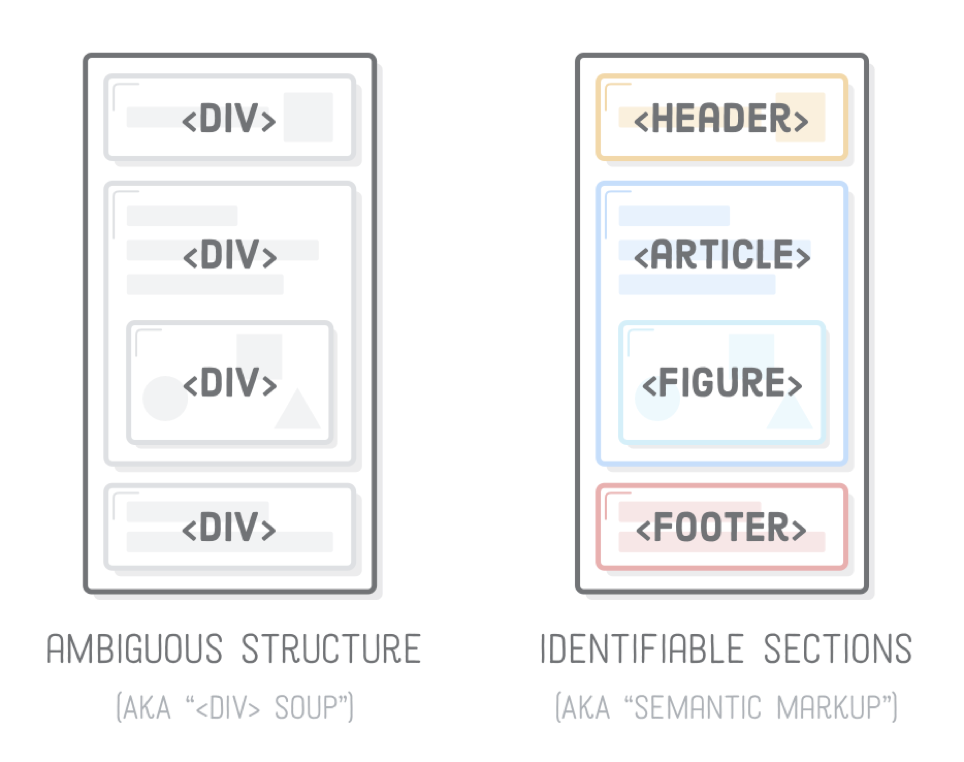
\includegraphics[width=0.8\textwidth]{figures/div-soup}
\label{fig:div-soup}
\caption{An illustration of the ambiguities that can arise when using Div elements to impose structure instead of HTML5 semantic elements.}
\end{figure}

\section{Structure \& Meaning}
\paragraph{} Let's take a slight detour and consider the relationship between the structure of a web page and the meaning of its content. If we consider a search engine, indexing all of the pages that it can find, so that it can show other people to it as necessary. A search engines doesn’t see the style and presentation of your page. It only sees the content. For efficiency, many search engines will ignore the CSS because the CSS isn't meant to convey meaning, only visual style and presentation, so can be safely ignored. Instead the HTML is interrogated, because the HTML is meant to convey meaning. The search engine will only care about the HTML because it is designed to attempt to "understand" the content and it is the HTML that holds the content. 

\paragraph{} Where we place content on a page, and how we mark it up, can alter how that content is dealt with. This is not from a visual presentation perspective, but from the internal structure and semantic meaning perspective. For example, content in an $<$h1$>$ tag is more likely to be weighted as important to interpreting the overall structure of a page, and as a result contributes to the search engine analysis of a page in a different way to other content marked up using the $<$p$>$ tag.

\section{Semantic Markup}
\paragraph{} Semantic markup stemmed from the drive towards marking up meaning in addition to the typographic elements that make up any given document. This happened in response to designers attempting to bring semantic markup to HTML. A good example is the use of $<$div$>$ and $<$span$>$ tags to group elements of a page together as we saw earlier when considering div soup. The main problem is that these $<$div$>$ and $<$span$>$ themselves don’t actually mean anything. They don't have any inherent meaning. If you are presented with a $<$div$>$ then it is difficult to infer exactly how the content of the <div> should be treated. For example, one $<$div$>$ could be a navigational collection, another $<$div$>$ could contain core content. How does a machine separate them so that it can treat each appropriately?

\paragraph{} By being explicit and including tags in HTML5 to support these goals we can use appropriate tags to delineate between, e.g. core content and navigation. The browser can then treat each differently as appropriate. This is why HTML5 includes tags like the  $<$nav$>$ tag, to communicate that its content should be treated as navigational content and not as body content or any other kind of content.

\paragraph{} Over the years, designers defined their own IDs and class names but this was ad hoc; people took their own approaches and so they were naturally inconsistent. This made pages difficult to process. For example, search engines detecting useful parts of a given page, or braille readers being able to ignore navigational elements when reading page content. In response HTML was extended and clarified to include tags that communicate more clearly defined meaning about their content. This is, in time, leading towards better structure for pages, as well as increased accessibility, and more reliable automated processing, maintainability, and reuse of web resources. 

\section{HTML5}

\paragraph{} Semantic meaning has always been present in HTML but is now, since HTML5, emphasised. HTML5 attempts to address this through addition of meaningful grouping tags so that the various parts of a page can be delineated and communicated more easily and reliably. These could be considered as "sectioning elements" or even as “divs but with added meaning”. 

\paragraph{} HTML5 includes support for the following semantic markup:
\begin{itemize}
\item $<$section$>$ - a thematic grouping of content, typically with a heading
\item $<$article$>$ - independent, self-contained content (suitable for syndication or reuse)
\item $<$header$>$ - container for introductory content
\item $<$footer$>$ - information about its containing element (author, copyright, \&c.)
\item $<$nav$>$ - major blocks of navigational links
\item $<$aside$>$ - related additional content
\item $<$figure$>$ \& $<$figcaption$>$ - visually explain an image
\item $<$main$>$ - the core content of the document
\item $<$mark$>$ - highlighted/emphasised sections
\item $<$details$>$ - additional information that can be hidden/shown
\item $<$summary$>$ - visible heading associated with $<$details$>$
\item $<$time$>$ - date/time information
\end{itemize}

\paragraph{} Most of these tags should have names that enable you to reasonably easily infer their intent. This is what makes them semantic tags. These new tags can be used to communicate the various parts of a page as shown in the following figure.

\begin{figure}[H]
\centering
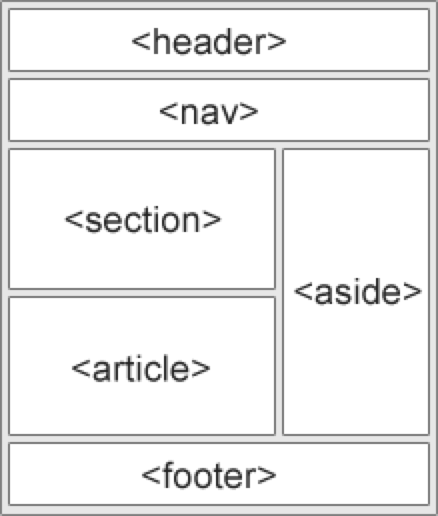
\includegraphics[width=0.8\textwidth]{figures/semantic-sections}
\label{fig:semantic-sections}
\caption{}
\end{figure}


\section{Semantic Meaning in Inherited Tags}
\paragraph{} The move to HTML5 involved some inherited pre-existing tags being redefined to have semantic meaning where previously they did not. This is summarised in the following table. You should notice the absence of the <b> and <i> tags - these have presentational meaning only so are not considered to be semantic HTML.


\begin{figure}[H]
\centering
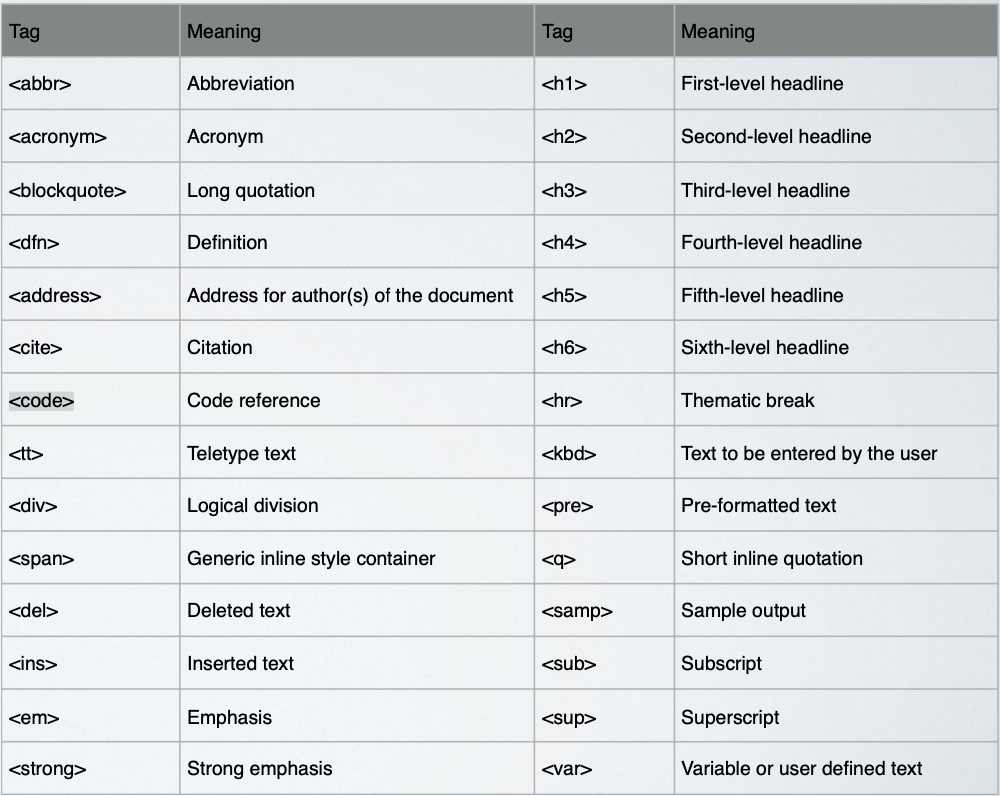
\includegraphics[width=0.8\textwidth]{figures/semantic-tags}
\label{fig:semantic-tags}
\caption{}
\end{figure}


\section{Summary}
\paragraph{} We've covered a lot of ground again in this unit. You should now: 

\begin{itemize}
\item understand how HTML has developed and why it works the way it does 
\item be aware of the range of tags supported by HTML 
\item be able to assemble basic HTML documents 
\item understand the difference between syntax and semantics
\item be aware of the need for semantic representation within markup
\item know about the range of semantic tags within HTML5
\end{itemize}
\paragraph{} There is obviously much more to effective HTML use than we can cover in one unit, but we can develop effective skills through practise. This isn’t the end of the story about HTML, semantics, and the representation and use of meaning on the Web, we’ll see HTML much more as we style and interact (programmatically) with it.

\paragraph{} For a diversion you could consider investigating the ``Semantic Web''. This is the ``web of meaning'' which is finding new application alongside AI technologies if you want to get an idea about one possible future of the Web.

